\documentclass[12pt,a4paper]{article}

% ============================================================
% FLUXX — CUHK-X LARGE MODEL TRACK TECHNICAL REPORT
% ============================================================

\usepackage[margin=0.83in,top=0.72in,bottom=0.78in]{geometry}
\usepackage{setspace}
\setstretch{1.5}

\usepackage{amsmath,amssymb}
\usepackage{booktabs}
\usepackage{array}
\usepackage{tabularx}
\usepackage{graphicx}
\usepackage{xcolor}
\usepackage{enumitem}
\usepackage{microtype}
\usepackage{titlesec}
\usepackage{fancyhdr}
\usepackage{tcolorbox}
\usepackage{tikz}
\usetikzlibrary{arrows.meta,positioning}
\usepackage[hidelinks]{hyperref}

% ============================================================
% Visual system
% ============================================================

\definecolor{FluxxNavy}{HTML}{14213D}
\definecolor{FluxxBlue}{HTML}{315B8A}
\definecolor{FluxxLight}{HTML}{F3F6F9}
\definecolor{FluxxGray}{HTML}{5E6875}
\definecolor{FluxxRule}{HTML}{D7DEE7}

\hypersetup{
    colorlinks=true,
    linkcolor=FluxxNavy,
    urlcolor=FluxxBlue,
    citecolor=FluxxBlue
}

\titleformat{\section}
{\large\bfseries\color{FluxxNavy}}
{\thesection}{0.55em}{}

\titleformat{\subsection}
{\normalsize\bfseries\color{FluxxBlue}}
{\thesubsection}{0.5em}{}

\titlespacing*{\section}{0pt}{1.0em}{0.35em}
\titlespacing*{\subsection}{0pt}{0.7em}{0.2em}

\setlength{\parindent}{0pt}
\setlength{\parskip}{0.34em}

\setlist[itemize]{
    leftmargin=1.35em,
    topsep=0.15em,
    itemsep=0.05em,
    parsep=0pt
}
\setlist[enumerate]{
    leftmargin=1.45em,
    topsep=0.15em,
    itemsep=0.08em,
    parsep=0pt
}

\renewcommand{\arraystretch}{1.13}

\pagestyle{fancy}
\fancyhf{}
\fancyhead[L]{\small\color{FluxxGray}\textbf{Fluxx} --- CUHK-X Large Model Track}
\fancyhead[R]{\small\color{FluxxGray}Technical Report}
\fancyfoot[C]{\small\color{FluxxGray}\thepage}
\renewcommand{\headrulewidth}{0.3pt}
\renewcommand{\headrule}{\hbox to\headwidth{\color{FluxxRule}\leaders\hrule height \headrulewidth\hfill}}

\newcommand{\method}{\textsc{Fluxx-SMR}}
\newcommand{\score}{\textbf{334/342}}
\newcommand{\pubscore}{\textbf{0.97660}}

\newtcolorbox{resultbox}{
    colback=FluxxLight,
    colframe=FluxxNavy,
    boxrule=0.6pt,
    arc=2pt,
    left=8pt,
    right=8pt,
    top=6pt,
    bottom=6pt
}

\newtcolorbox{insightbox}{
    colback=white,
    colframe=FluxxRule,
    boxrule=0.45pt,
    arc=2pt,
    left=8pt,
    right=8pt,
    top=5pt,
    bottom=5pt
}

% ============================================================
\begin{document}
% ============================================================

% ============================================================
% Title
% ============================================================

{\color{FluxxNavy}\rule{\textwidth}{2.1pt}}

\vspace{0.45em}

{\LARGE\bfseries
Structure Before Scale
}

\vspace{0.15em}

{\large\bfseries\color{FluxxBlue}
Constraint-Guided Multimodal Reasoning for Privacy-Preserving Human Activity Understanding
}

\vspace{0.6em}

\begin{tabularx}{\textwidth}{@{}>{\bfseries}l X >{\bfseries}l X@{}}
Team & Fluxx &
Track & Large Model Track \\

Member & Toheeb Goodluck Ogunade &
Kaggle team & Fluxx \\

Email & \texttt{ogunadetoheeb4@gmail.com} &
Faculty advisor & N/A
\end{tabularx}

\vspace{0.45em}

\begin{resultbox}
\textbf{Final public result:}
\score{} = \pubscore.

\textbf{Selected Kaggle submissions:}
\texttt{56239239} (keeper, 334/342) and
\texttt{56250404} (private lottery ticket, 334/342);
both reproduced byte-identically (Section~7).

\textbf{Core result:}
a compact, fully reproducible multimodal system reached within
\textbf{three public answers} of the leading 337/342 score without a
closed-source API or monolithic large vision-language model.
\end{resultbox}

% ============================================================
\section{One-Paragraph Summary}
% ============================================================

We present \method{} (Session-state Multimodal Reasoning), a structure-first
system for the CUHK-X Large Model Track \cite{cuhkx}.
Our central idea is that the benchmark should not be treated as hundreds of
independent multimodal question-answering problems. Multiple questions often
describe the same underlying recording session and therefore constrain a shared
latent physical state: which actions occurred, which objects were manipulated,
how actions were ordered, and how they were performed. We first extract compact
evidence from skeleton trajectories, IMU and radar streams, and committed
temporal action logits, then reconstruct the session state and jointly solve
related questions under explicit consistency constraints. Lightweight
specialists handle residual object, sequence, combination and manner cases
only when subject-disjoint validation shows positive incremental value over
the existing system. The final pipeline uses committed sensor features and
small trained heads rather than a frontier VLM or any loaded visual backbone,
yet achieved \score{} public accuracy. We attribute this
performance to moving model capacity away from repeatedly rediscovering the
same event and toward explicit inference over the structure already present in
the multimodal task.

% ============================================================
\section{Method Overview}
% ============================================================

\subsection{Problem factorization}

A conventional formulation predicts each answer independently,

\[
    \hat{y}_q = f(x_q,q,\mathcal{O}_q),
\]

where \(x_q\) is the multimodal clip, \(q\) the question and
\(\mathcal{O}_q\) its answer options.

We instead introduce a latent session state

\[
    z_s = (A_s,\pi_s,O_s,M_s),
\]

where

\[
    A_s = \text{actions},\qquad
    \pi_s = \text{temporal order},\qquad
    O_s = \text{objects},\qquad
    M_s = \text{manner/style}.
\]

Questions associated with session \(s\) become partial observations of the same
\(z_s\). Single-action questions constrain \(A_s\); combination questions
constrain subsets of \(A_s\); ordering questions constrain \(\pi_s\); and object
or manner questions constrain \(O_s\) and \(M_s\).

The problem is therefore closer to

\[
    \boxed{
    \text{multimodal evidence}
    \rightarrow
    \text{latent session reconstruction}
    \rightarrow
    \text{consistent answers}
    }
\]

than to independent end-to-end VQA.

\subsection{Top-down system flow}

\begin{figure}[ht]
\centering

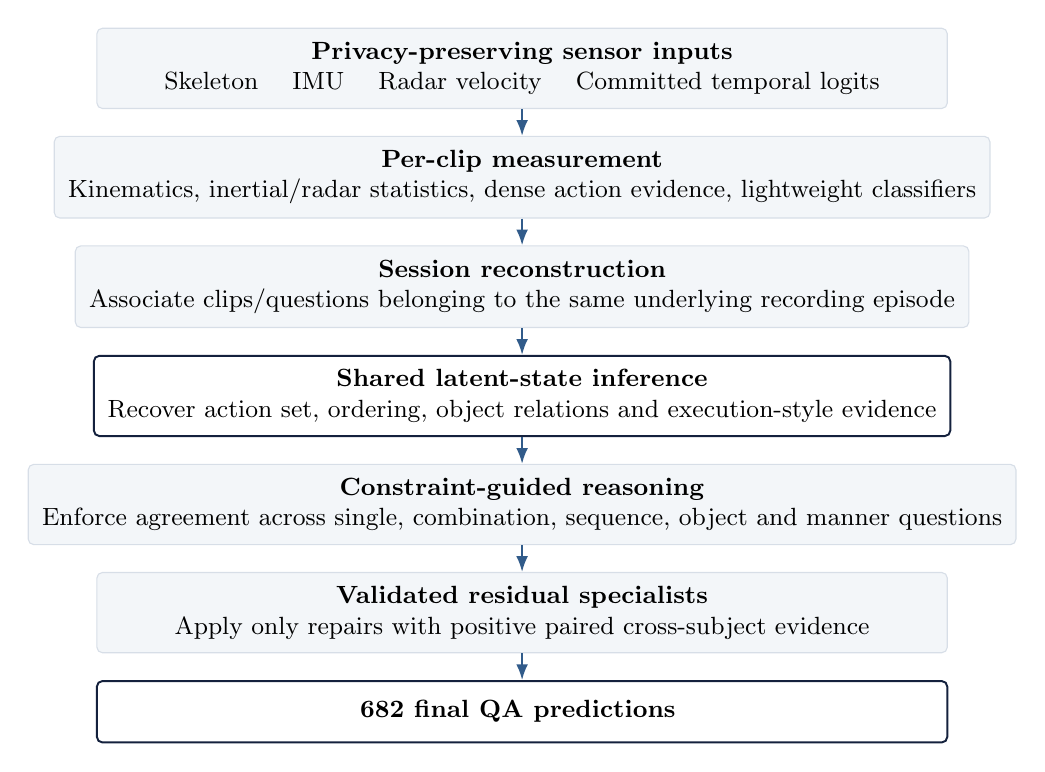
\begin{tikzpicture}[
    node distance=0.34cm,
    every node/.style={font=\small},
    stage/.style={
        rectangle,
        rounded corners=2pt,
        draw=FluxxRule,
        fill=FluxxLight,
        minimum width=10.8cm,
        minimum height=0.72cm,
        align=center,
        inner sep=5pt
    },
    strong/.style={
        rectangle,
        rounded corners=2pt,
        draw=FluxxNavy,
        fill=white,
        line width=0.7pt,
        minimum width=10.8cm,
        minimum height=0.78cm,
        align=center,
        inner sep=5pt
    },
    arrow/.style={
        -{Latex[length=2mm]},
        line width=0.7pt,
        color=FluxxBlue
    }
]

\node[stage] (raw) {
\textbf{Privacy-preserving sensor inputs}\\
Skeleton \quad IMU \quad Radar velocity \quad Committed temporal logits
};

\node[stage, below=of raw] (measure) {
\textbf{Per-clip measurement}\\
Kinematics, inertial/radar statistics, dense action evidence, lightweight classifiers
};

\node[stage, below=of measure] (group) {
\textbf{Session reconstruction}\\
Associate clips/questions belonging to the same underlying recording episode
};

\node[strong, below=of group] (latent) {
\textbf{Shared latent-state inference}\\
Recover action set, ordering, object relations and execution-style evidence
};

\node[stage, below=of latent] (constraints) {
\textbf{Constraint-guided reasoning}\\
Enforce agreement across single, combination, sequence, object and manner questions
};

\node[stage, below=of constraints] (repair) {
\textbf{Validated residual specialists}\\
Apply only repairs with positive paired cross-subject evidence
};

\node[strong, below=of repair] (out) {
\textbf{682 final QA predictions}
};

\draw[arrow] (raw) -- (measure);
\draw[arrow] (measure) -- (group);
\draw[arrow] (group) -- (latent);
\draw[arrow] (latent) -- (constraints);
\draw[arrow] (constraints) -- (repair);
\draw[arrow] (repair) -- (out);

\end{tikzpicture}

\caption{
\method{} separates perception from reasoning.
Modalities estimate physical evidence; session-level structure converts that
evidence into globally consistent answers.
}
\end{figure}

\subsection{Structural objective}

Conceptually, session inference solves

\[
z_s^\star
=
\arg\max_{z_s\in\mathcal{Z}_s}
\sum_r
w_r\,
\phi_r(z_s;x_s)
\quad
\text{s.t.}
\quad
C_j(z_s)=1,
\]

where \(\phi_r\) is evidence from modality or specialist \(r\), and \(C_j\)
represents structural constraints induced by the related questions.

The distinction is important: our learned models estimate uncertain physical
quantities; deterministic reasoning enforces relationships that do not need to
be relearned from data.

% ============================================================
\section{Modalities and Model Design}
% ============================================================

\subsection{Modalities}

\begin{table}[ht]
\centering
\small
\begin{tabularx}{\textwidth}{
    >{\bfseries}p{1.55cm}
    p{1.0cm}
    p{4.1cm}
    X
}
\toprule
Modality & Used & Representation & Primary role \\
\midrule

Skeleton &
Yes &
Joint trajectories, relative geometry and temporal kinematics &
High-signal representation of body motion; supports action and temporal reasoning. \\

IMU &
Yes &
Synchronized inertial channels, magnitudes and temporal derivatives &
Direct physical evidence of motion dynamics independent of appearance. \\

Depth &
No &
Evaluated via frozen encoders during development; not loaded at inference &
No solver code path reads depth features in the frozen system. \\

Thermal &
No &
Evaluated during development; not loaded at inference &
Same as depth: explored, then excluded from the final path. \\

Infrared &
No &
N/A &
Explored during development but not required by the final selected decision path. \\

mmWave / radar &
Yes &
\texttt{rad\_*} velocity statistics in the committed feature cache &
Active input to block features and action classifiers. \\

\bottomrule
\end{tabularx}
\caption{Modalities in the final reproducible pipeline.}
\end{table}

\subsection{Learned components}

The system does not have one monolithic base model. Its learned components are
deliberately small and all ship as committed data rather than weight files:

\begin{itemize}
    \item committed dense temporal action logits (skeleton+IMU model, frozen as per-clip log-probabilities);
    \item a committed HARn action log-probability cache from gradient-boosted trees over skeleton/IMU/radar statistics \cite{sklearn};
    \item small gradient-boosting / logistic-regression heads, fit on the frozen training features at run time (seconds on CPU).
\end{itemize}

Frozen DINOv2 ViT-S/14 \cite{dinov2} and MobileNetV3-Small \cite{mobilenetv3}
were evaluated as \emph{measurement devices}, not question-answering engines:
they never receive the natural-language question. Three early lineage rows
trace to DINO-assisted evidence, but the frozen inference path loads no
backbone weights at all (verified: the archived outputs reproduce byte-identically
with all visual-feature files removed).

Fusion occurs at the evidence and decision levels (log-probability mixing under
session constraints) rather than through raw token concatenation.

\subsection{Question-specific reasoning}

\textbf{Single action.}
Per-clip sensor scores are restricted to the session's feasible action set,
with pool-membership bonuses breaking ties between kinematically similar actions.

\textbf{Combination / multi-action.}
Candidate co-occurrence is reconciled with actions inferred from sibling
questions in the same session; exact-set answers must match the pool exactly.

\textbf{Sequence.}
Dense temporal evidence proposes an ordering via monotone decoding, while
action identity and session constraints veto structurally incompatible
permutations; the final correction was isolated by bisecting a candidate bundle.

\textbf{Object.}
Object predictions are coupled to the action being performed through
object$\leftrightarrow$single consistency checks over stable action--object
co-occurrence.

\textbf{Emotion / manner.}
Execution-style reasoning runs only after action identity is established,
separating ``what happened'' from ``how it happened,'' with exact donor
templates resolving the remaining cases.

% ============================================================
\section{Data Sources and Usage}
% ============================================================

\begin{table}[ht]
\centering
\small
\begin{tabularx}{\textwidth}{
    p{3.35cm}
    p{2.1cm}
    X
    p{2.15cm}
}
\toprule
\textbf{Source} & \textbf{Type} & \textbf{Use} & \textbf{Stage} \\
\midrule

CUHK-X training data &
Official &
Training labels, sensor streams, QA structure and cross-subject validation &
Training / validation \\

CUHK-X test data &
Official &
Label-free multimodal inference &
Inference \\

DINOv2 ViT-S/14 &
Public pretrained &
Frozen image features (evaluated; 3 historical lineage rows) &
Development only \\

MobileNetV3-Small &
Public pretrained &
Frozen lightweight features (evaluated, unused) &
Development only \\

Committed feature caches &
Derived, frozen &
Skeleton/IMU/radar stats, dense logits, HARn log-probs &
Inference \\

External labelled data &
N/A &
None &
N/A \\

Synthetic/pseudo-labelled data &
N/A &
None in final system &
N/A \\

Closed-source API &
N/A &
None &
N/A \\

\bottomrule
\end{tabularx}
\caption{All data and pretrained sources that affect the final pipeline.}
\end{table}

No external labelled dataset or closed-source service is required.

Preprocessing consists of deterministic modality loading, clip/session
association, skeleton/IMU feature construction, frame normalization, temporal
aggregation and explicit handling of missing signals.

A final-day audit discovered that a skeleton filename parser rejected a valid
short-filename pattern. Fixing the parser restored the appropriate physical
evidence and improved the public score by one answer. This fix was generic
data plumbing rather than test-specific relabelling.

% ============================================================
\section{Training, Validation, and Generalization}
% ============================================================

\subsection{Cross-subject protocol}

The dominant expected distribution shift is to unseen people. We therefore
avoid random row-level validation and use five-fold subject-disjoint OOF
evaluation: every example belonging to one subject remains in the same fold.

The canonical fold construction uses seed \(7\).

The faithfully reconstructed OOF system obtained

\[
    3841/4087 = 94.00\%.
\]

The final public leaderboard result was

\[
    334/342 = 97.66\%.
\]

The gap is expected and audited rather than a sign of overfitting: the OOF
number evaluates the pipeline \emph{before} the frozen correction lineage,
while the public score includes 51 documented per-row corrections (36
mechanism patches, 13 pinned validated values, 2 probed singletons), each
traceable to subject-disjoint OOF evidence, a validating live probe, or a
pinned validated value. The lineage is a fixed, pre-registered correction
layer, not test-time tuning.

\begin{table}[ht]
\centering
\small
\begin{tabularx}{\textwidth}{p{5.1cm}X}
\toprule
\textbf{Item} & \textbf{Result} \\
\midrule

Validation type &
5-fold cross-subject / leave-whole-users-out \\

Held-out subjects &
Every training subject is held out exactly once \\

Canonical seed &
7 \\

Faithful local OOF (pre-lineage pipeline) &
3841/4087 = 94.00\% \\

Public leaderboard (pipeline + 51-row lineage) &
334/342 = 97.66\% \\

Observed difference &
Public accuracy is 3.66 percentage points above faithful OOF;
the lineage, not overfitting, explains it \\

Expected unseen-subject behaviour &
Strong relative robustness because component promotion was subject-disjoint \\

Primary distribution-shift concern &
Sensor synchronization, acquisition protocol, metadata/session semantics and sensor calibration \\

\bottomrule
\end{tabularx}
\caption{Validation and expected generalization.}
\end{table}

\subsection{Incremental validation}

A major methodological lesson was that standalone accuracy is not sufficient
for a mature system.

For every proposed specialist, we measure only the rows it would change:

\[
\Delta
=
N_{W\rightarrow R}
-
N_{R\rightarrow W},
\]

where \(W\rightarrow R\) counts incumbent errors corrected by the candidate and
\(R\rightarrow W\) counts correct incumbent answers it breaks. Only
\(\Delta > 0\) under subject-disjoint evaluation justifies promotion.

A new component is useful only if it knows something the existing system does
not already know.

\begin{insightbox}
\textbf{Promotion principle.}
We do not ask whether a new model is accurate in isolation.
We ask whether it provides \emph{incremental information} over the strongest
existing system under subject-disjoint evaluation.
\end{insightbox}

% ============================================================
\section{Results and Evidence}
% ============================================================

\subsection{Final result}

\[
\boxed{
334/342 = 97.660\%
}
\]

At freeze time, the leading public score was \(337/342\). The gap was therefore

\[
3/342 = 0.877\%.
\]

\subsection{Champion lineage}

\begin{table}[ht]
\centering
\small
\begin{tabular}{lccc}
\toprule
\textbf{System} & \textbf{Correct} & \textbf{Score} & \textbf{Net} \\
\midrule
Protected champion & 332/342 & 0.97076 & --- \\
Skeleton-path repair & 333/342 & 0.97368 & +1 \\
Final sequence correction & \textbf{334/342} & \textbf{0.97660} & +1 \\
\bottomrule
\end{tabular}
\caption{Final public-score lineage.}
\end{table}

The first gain came from the generic skeleton-path bug fix. The second came
from decomposing a sequence candidate and isolating the ordering supported by
the strongest available evidence. Kaggle refs: \texttt{56090799} $\rightarrow$
\texttt{56238613} $\rightarrow$ \texttt{56239239}.

\subsection{Negative result I: temporal TCN}

One of our most useful failures was a dilated temporal convolutional network
over skeleton and IMU signals.

On an early reconstructed sequence benchmark it appeared dramatically better:

\[
37.7\%
\rightarrow
55.7\%.
\]

Yet applying its 21 test-time sequence changes moved the public score from

\[
332
\rightarrow
322.
\]

A separately selected high-confidence subset also regressed to 329.

The failure exposed a validation flaw: the TCN had beaten a weaker reconstructed
sequence surrogate, not the actual champion's complete structural decision
path.

After this result, all specialists were required to beat the actual component
they intended to replace.

\subsection{Negative result II: stronger visual embeddings}

We also tested a late frozen DINOv2 visual specialist (ViT-S/14 stride-1
color embeddings, full-frame plus actor crop, with a ViT-B/14 ablation over
1007 clips). On matched OOF pool predictions:

\begin{table}[ht]
\centering
\small
\begin{tabular}{lcc}
\toprule
\textbf{Target} & \textbf{Late DINO specialist} & \textbf{Existing system} \\
\midrule
Single-action pool & 67.5\% & 99.9\% \\
Multi-action pool & 15\% & 97\% \\
Combination pool & 0\% & 99\% \\
\bottomrule
\end{tabular}
\caption{Matched comparison of the late DINO override branch.}
\end{table}

The experiment produced no DINO-only correction worth shipping.

A separate nested HARn experiment showed an approximately \(+4\%\) fusion gain,
but that improvement lived inside a weaker intermediate component and did not
translate into a trustworthy final-answer override.

The late DINO override branch therefore contributed \textbf{zero final flips}.

This does not imply that DINO representations are intrinsically weak; rather,
the existing structural system had already captured the information relevant to
the affected rows.

\subsection{What actually mattered}

Our strongest gains came from four properties:

\begin{enumerate}
    \item \textbf{Sensor-native representations.}
    Skeleton and IMU expose physical motion directly.

    \item \textbf{Shared latent state.}
    Several QA rows often describe the same underlying activity episode.

    \item \textbf{Explicit consistency.}
    Related answers cannot contradict one another.

    \item \textbf{Conservative residual correction.}
    Specialists are used only where they outperform the existing system
    conditionally, not merely globally.
\end{enumerate}

% ============================================================
\section{Efficiency and Reproducibility}
% ============================================================

\subsection{Compute profile}

\begin{table}[ht]
\centering
\small
\begin{tabularx}{\textwidth}{p{5.3cm}X}
\toprule
\textbf{Item} & \textbf{Final system} \\
\midrule

Development GPU (research only) &
NVIDIA Tesla P100 16GB on Kaggle; largest visual-extraction run $\approx$ 2.6 GPU-hours \\

Inference GPUs required &
0 (CPU-only; solver pins torch to CPU/MPS, no CUDA calls) \\

Peak GPU memory (inference) &
0 GB \\

Peak host RAM (inference) &
\(\leq 4\) GB (full run verified on a 2~GB CPU box) \\

End-to-end inference runtime &
\(\approx\) 1--3 minutes single-threaded for 682 answers \\

Task-specific training cost &
Runtime sklearn fits in seconds; all heavy features precomputed and committed \\

Checkpoint/package size &
\(\approx\) 80~MB committed caches + code (below 1~GB excluding official bulk data) \\

Custom CUDA/C++ extensions &
None \\

FlashAttention / xformers / bitsandbytes &
None \\

DeepSpeed / vLLM / SGLang / Apex &
None \\

Closed-source inference API &
None \\

\bottomrule
\end{tabularx}
\caption{Compute and dependency profile.}
\end{table}

\subsection{Exact final artifact}

Primary selected submission:

\begin{verbatim}
submission_097660_334of342_CHAMPION.csv
\end{verbatim}

Kaggle submission ID:

\begin{verbatim}
56239239
\end{verbatim}

SHA-256:

\begin{verbatim}
1ea4bf7e1eae01c7ed5475dd9e358fbbed4f1f1804c853b88ee86f1da89f83e4
\end{verbatim}

The file contains exactly 682 unique \texttt{qa\_id} rows.

Second selected submission (private lottery ticket,
\texttt{submissions/V2\_flipall\_coins.csv}, ref \texttt{56250404}):
334/342 with three flips on pigeonhole-proved private rows
(\texttt{test\_0526} D$\rightarrow$A, \texttt{test\_0432} C$\rightarrow$B,
\texttt{test\_0456} C$\rightarrow$A). SHA-256:

\begin{verbatim}
9c63f82a34e6ac982054fcbfc80a815c60fb7c2152f6bf68f4b48f30fbeec072
\end{verbatim}

Both variants are reproduced by the same script (variant flag below) and
verified byte-identical against these hashes.

\subsection{Reproduction package}

\begin{table}[ht]
\centering
\small
\begin{tabularx}{\textwidth}{p{4.8cm}X}
\toprule
\textbf{Artifact} & \textbf{Location / description} \\
\midrule

Source repository &
\texttt{qeinstein/cuchx-large} \\

Entry point &
\texttt{inference.sh} \\

Main command &
\texttt{bash inference.sh <data\_dir> <output\_csv> [334|flipall]} \\

Variant configs &
\texttt{repro/variant\_334.json}, \texttt{repro/variant\_flipall.json} \\

Byte-verifier &
\texttt{python3 repro/verify.py --variant <v> --got <csv>} \\

Environment specification &
\texttt{requirements.txt} (numpy/pandas/sklearn/scipy/torch-CPU, pinned) \\

Run guide &
\texttt{repro/README.md} \\

Method documentation &
\texttt{README.md} \\

Submission provenance &
\texttt{repro/SUBMISSION\_RECORD.md} \\

External-data disclosure &
\texttt{repro/EXTERNAL\_DATA.md} \\

Final artifacts &
\texttt{submissions/submission\_097660\_334of342\_CHAMPION.csv} and
\texttt{submissions/V2\_flipall\_coins.csv} \\

Internet requirement &
None: no downloads at inference (all features are committed caches) \\

\bottomrule
\end{tabularx}
\caption{Reproduction package contents.}
\end{table}

The committee reproduction procedure is:

\begin{enumerate}
    \item clone or unpack the exact frozen repository revision;
    \item create the pinned Python environment (\texttt{pip install -r requirements.txt});
    \item run, once per selected variant,
\begin{verbatim}
bash inference.sh <data_dir> out_334.csv 334
bash inference.sh <data_dir> out_flipall.csv flipall
\end{verbatim}
    \item verify row-for-row and SHA-256 equality with the archived artifacts:
\begin{verbatim}
python3 repro/verify.py --variant 334 --got out_334.csv
python3 repro/verify.py --variant flipall --got out_flipall.csv
\end{verbatim}
\end{enumerate}

The input path is supplied at runtime and is not hard-coded. No step requires
network access.

% ============================================================
\section{Large Model Track Characteristics}
% ============================================================

\begin{table}[ht]
\centering
\small
\begin{tabularx}{\textwidth}{p{5.0cm}X}
\toprule
\textbf{Item} & \textbf{Final answer} \\
\midrule

Base model &
No monolithic LLM/VLM \\

Visual backbones &
DINOv2 ViT-S/14 ($\approx$21M) and MobileNetV3-Small: evaluated frozen,
not loaded at inference \\

Backbone weights loaded &
None (all visual evidence excluded or committed as data) \\

Closed-source/API &
No \\

LLM prompting &
N/A \\

LoRA/adapters &
N/A in final system \\

Non-RGB handling &
Skeleton, IMU and radar stay numerical (engineered statistics + committed
logits); depth/thermal/infrared evaluated but excluded from the final path \\

Fusion &
Late evidence fusion followed by session-level structural reasoning \\

Primary inference cost &
Small sklearn fits plus session solve; minutes on CPU, no GPU stage \\

\bottomrule
\end{tabularx}
\caption{Large Model Track implementation summary.}
\end{table}

\subsection{Why a small system can be competitive}

Our result should not be interpreted as evidence that small neural networks are
generally as capable as frontier multimodal models.

The more specific explanation is that CUHK-X provides several modalities that
already expose the relevant physical variables directly.

A generic visual model must infer pose and motion from pixels. Skeleton and IMU
instead provide quantities close to

\[
\{p_j(t)\}_{j=1}^{J},
\qquad
a(t),
\qquad
\omega(t),
\]

where \(p_j(t)\) denotes joint position and \(a(t),\omega(t)\) inertial motion.

The remaining difficulty is therefore less about reconstructing reality from
appearance and more about combining noisy observations consistently.

The second advantage is redundancy. Once a session's latent action state has
been recovered, several QA answers become consequences of the same state.

Our system therefore follows the principle

\[
\boxed{
\text{learn uncertain perception}
\;+\;
\text{encode known structure explicitly}
}
\]

rather than asking one large model to relearn both.

% ============================================================
\section{Limitations and Lessons Learned}
% ============================================================

\subsection{Main limitation}

The strongest assumption in \method{} is that the relation between clips,
sessions and question families remains similar under evaluation.

If the acquisition protocol changes enough that this shared structure
disappears, the benefit of joint reasoning will decrease.

\subsection{Distribution shifts of greatest concern}

We expect subject identity shift to be less damaging than:

\begin{itemize}
    \item changed sensor calibration;
    \item degraded skeleton extraction;
    \item changed IMU orientation or sampling;
    \item cross-modal desynchronization;
    \item altered session construction;
    \item systematic missing modalities.
\end{itemize}

\subsection{Lessons from failed models}

\textbf{1. Better standalone accuracy is not necessarily better system accuracy.}

A component matters only if it corrects residual incumbent errors.

\textbf{2. Validation must reproduce the system being replaced.}

The TCN failure was primarily a baseline-fidelity failure.

\textbf{3. At saturation, software correctness becomes a modeling issue.}

One of our final two public gains came from a filename parser defect rather than
a new architecture.

\textbf{4. Neutral leaderboard evidence skews private.}

Six elimination-backed rows that never moved the public score all proved to be
private-split rows once every option was tried. Surviving incumbent errors
concentrate where feedback cannot see them, so late-stage probing must discount
``neutral'' as evidence of absence.

\subsection{What we would do with one additional week}

The highest-value extension would be a learned \textbf{cross-modal residual verifier}.

Rather than replacing the existing solver, it would estimate

\[
P(\text{incumbent wrong}\mid
\text{sensor disagreement},
\text{confidence},
\text{question type},
\text{structural evidence}).
\]

Its features would include modality-specific probabilities, margins, entropy,
session consistency, specialist agreement and contradiction indicators.

The objective would be \emph{high-precision error detection}, not another
global classifier.

A second extension would replace parts of the deterministic session solver with
a probabilistic factor graph, preserving the same interpretable latent variables
while representing uncertainty more explicitly.

% ============================================================
\section{Conclusion}
% ============================================================

\method{} reached \score{} public accuracy using a compact, reproducible system
with no closed-source API and no monolithic VLM.

The result came from a particular division of labour:

\[
\boxed{
\begin{array}{c}
\text{Sensors estimate what physically happened} \\[0.2em]
\downarrow \\[-0.1em]
\text{Session inference reconstructs the shared event} \\[0.2em]
\downarrow \\[-0.1em]
\text{Constraints enforce consistency} \\[0.2em]
\downarrow \\[-0.1em]
\text{Specialists resolve validated residuals}
\end{array}}
\]

The most important finding was not that small models universally outperform
large ones. It was that \textbf{model scale is an inefficient substitute for
known problem structure}.

Skeleton, IMU and radar measurements already expose much of the physical
event. Once those signals are organized around a shared latent session state,
explicit reasoning can recover information that independent question-by-question
prediction discards.

Our development process produced the same lesson from the opposite direction:
both a stronger visual specialist and a temporal neural model looked promising
under narrower evaluations but failed to improve the complete system.

The final principle is therefore simple:

\begin{resultbox}
\centering
\textbf{Learn what is uncertain. Encode what is known.\\
Evaluate every new model by what it adds to the system, not by what it can do alone.}
\end{resultbox}

% ============================================================
\section{References}
% ============================================================

\begin{thebibliography}{9}

\bibitem{cuhkx}
S. Jiang, M. Yuan, X. Ji, B. Yang, Z. Liu, L. Xu, Y. Li, Y. He,
L. Dong, W. Lu, Z. Yan, X. Jiang, W. Gao, H. Chen, and G. Xing,
``A Large-Scale Multimodal Dataset and Benchmarks for Human Activity
Scene Understanding and Reasoning,''
\textit{Proceedings of the 24th Annual International Conference on Mobile
Systems, Applications and Services (MobiSys '26)}, 2026.

\bibitem{dinov2}
M. Oquab et al.,
``DINOv2: Learning Robust Visual Features without Supervision,''
\textit{Transactions on Machine Learning Research}, 2024.

\bibitem{mobilenetv3}
A. Howard et al.,
``Searching for MobileNetV3,''
\textit{Proceedings of the IEEE/CVF International Conference on Computer
Vision}, 2019.

\bibitem{sklearn}
F. Pedregosa et al.,
``Scikit-learn: Machine Learning in Python,''
\textit{Journal of Machine Learning Research},
vol. 12, pp. 2825--2830, 2011.

\end{thebibliography}

\end{document}
